%=======================02-713 LaTeX template, following the 15-210 template==================
%
% You don't need to use LaTeX or this template, but you must turn your homework in as
% a typeset PDF somehow.
%
% How to use:
%    1. Update your information in section "A" below
%    2. Write your answers in section "B" below. Precede answers for all 
%       parts of a question with the command "\question{n}{desc}" where n is
%       the question number and "desc" is a short, one-line description of 
%       the problem. There is no need to restate the problem.
%    3. If a question has multiple parts, precede the answer to part x with the
%       command "\part{x}".
%    4. If a problem asks you to design an algorithm, use the commands
%       \algorithm, \correctness, \runtime to precede your discussion of the 
%       description of the algorithm, its correctness, and its running time, respectively.
%    5. You can include graphics by using the command \includegraphics{FILENAME}
%
\documentclass[11pt]{article}
\usepackage{amsmath,amssymb,amsthm}
\usepackage{graphicx}
\usepackage[margin=1in]{geometry}
\usepackage{fancyhdr}
\usepackage{tikz}
\usetikzlibrary{automata, positioning, arrows, calc}
\tikzset{
	% ->, % makes the edges directed
	% >=stealth’, % makes the arrow heads bold
	node distance=3cm, % specifies the minimum distance between two nodes. Change if necessary.
	every state/.style={thick, fill=gray!10}, % sets the properties for each ’state’ node
	initial text=$ $, % sets the text that appears on the start arrow
	every loop/.style={}, % removes the arrow from the loops
}
\tikzset{me/.style={to path={
\pgfextra{% 
 \pgfmathsetmacro{\startf}{-(#1-1)/2}  
 \pgfmathsetmacro{\endf}{-\startf} 
 \pgfmathsetmacro{\stepf}{\startf+1}}
 \ifnum 1=#1 -- (\tikztotarget)  \else
     let \p{mid}=($(\tikztostart)!0.5!(\tikztotarget)$) 
         in
\foreach \i in {\startf,\stepf,...,\endf}
    {%
     (\tikztostart) .. controls ($ (\p{mid})!\i*6pt!90:(\tikztotarget) $) .. (\tikztotarget)
      }
      \fi   
     \tikztonodes
}}}
\newtheorem{theorem}{Theorem}
\newtheorem{conjecture}{Conjecture}
\setlength{\parindent}{0pt}
\setlength{\parskip}{5pt plus 1pt}
\setlength{\headheight}{13.6pt}
\newcommand\question[2]{\vspace{.25in}\hrule\textbf{#1}: #2\vspace{.5em}\hrule\vspace{.10in}}
\renewcommand\part[1]{\vspace{.10in}(#1)\par}
\newcommand\algorithm{\vspace{.10in}\textbf{Algorithm: }}
\newcommand\correctness{\vspace{.10in}\textbf{Correctness: }}
\newcommand\runtime{\vspace{.10in}\textbf{Running time: }}
\newcommand{\R}{\mathbb{R}}
\newcommand{\N}{\mathbb{N}}
\newcommand{\Z}{\mathbb{Z}}
\pagestyle{fancyplain}
\lhead{\textbf{\NAME}}
\chead{\textbf{{\COURSE} Lesson \HWNUM \text{ }Exercises}}
\rhead{\today}
\begin{document}\raggedright
%Section A==============Change the values below to match your information==================
\newcommand\NAME{Eric Altenburg}  % your name
\newcommand\COURSE{MA-240}
\newcommand\HWNUM{15}              % the homework number
%Section B==============Put your answers to the questions below here=======================

% no need to restate the problem --- the graders know which problem is which,
% but replacing "The First Problem" with a short phrase will help you remember
% which problem this is when you read over your homeworks to study.

\textbf{Pledge:} \textit{I pledge my honor that I have abided by the Stevens Honor System.} -Eric Altenburg

\question{1}{Give an example of a graph that has an Euler path but not an Euler circuit.}
Figure~\ref{ep_nec} is an example of a graph with an Euler path but not an Euler circuit because the only traversals possible are $a \rightarrow b$ or $b \rightarrow a$. In both scenarios the start and end nodes are different, all while traversing each edge exactly once.
\begin{figure}[ht]
	\centering
	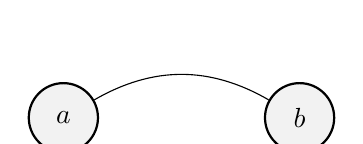
\begin{tikzpicture}
		\node[state] (left_node) {$a$};
		\node[state, right of=left_node] (right_node) {$b$};
		\draw (left_node) edge[bend left] (right_node);
	\end{tikzpicture}
	\caption{Graph with an Euler path but not an Euler circuit.}
	\label{ep_nec}
\end{figure}

\question{2}{Formulate a conjecture about which graphs admit an Euler path. You may wish to experiment by drawing different graphs, trying to draw an Euler path, and consider the properties of the graph. Then write down some ideas for proving your conjecture, and be prepared to explain them in class.}

\begin{conjecture}
	If a graph $G$ has exactly 2 vertices with odd degrees, then it has an Euler path.
\end{conjecture}

I'm not sure how to \textit{formally} prove this other than by talking through it. However, we know that ignoring beginning and end vertices, we know that any other vertex must have an edge that can let you reach it while also having an edge that allows you to leave it. This means any vertex that isn't the beginning or end must have an even degree. And because you begin and end at different points, it must be that there is one extra edge leaving the beginning node than there are those that lead to it. To end on a specific node that is not the beginning, the end node must have one less edge that leads to it than those that can lead away from it. This gives two nodes that must have an odd degree as shown in Figure~\ref{numtwo}.

\begin{figure}[ht]
	\centering
	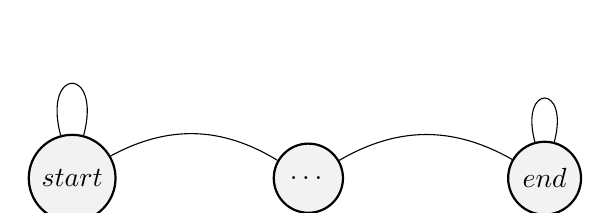
\begin{tikzpicture}
		\node[state] (start_node) {$start$};
		\node[state, right of=start_node] (middle_nodes) {\ldots};
		\node[state, right of=middle_nodes] (end_node) {$end$};

		\draw 	(start_node) edge[loop above] (start_node)
				(start_node) edge[bend left] (middle_nodes)
				(middle_nodes) edge[bend left] (end_node)
				(end_node) edge[loop above] (end_node);
	\end{tikzpicture}
	\caption{Graph demonstrating the proof idea.}
	\label{numtwo}
\end{figure}


\question{3}{Consider the house whose floor plan is shows below. Starting from any of the rooms or the outside, can you take a tour of the house that involves walking through each doorway exactly once? Explain.}

Taking a tour of the house while going through each doorway is another way of saying that there exists either a Euler path or circuit. By drawing the floor plan as a graph, we can then inspect each vertex to see its degrees. If every vertex has an even degree, then it has a circuit. If exactly 2 vertices have odd degrees, then it has a path. 

As seen in Figure~\ref{floorplan}, vertex $a$ has a degree of 9 so this eliminates the possibility of an Euler circuit. Vertex $e$ has a degree of 5 and $c$ has a degree of 5 as well. Because more than 2 vertices have an odd degree count, an Euler path is not possible either. Therefore, because neither traversals is possible, taking a tour by going through every door once is not possible.

\begin{figure}[ht]
	\centering
	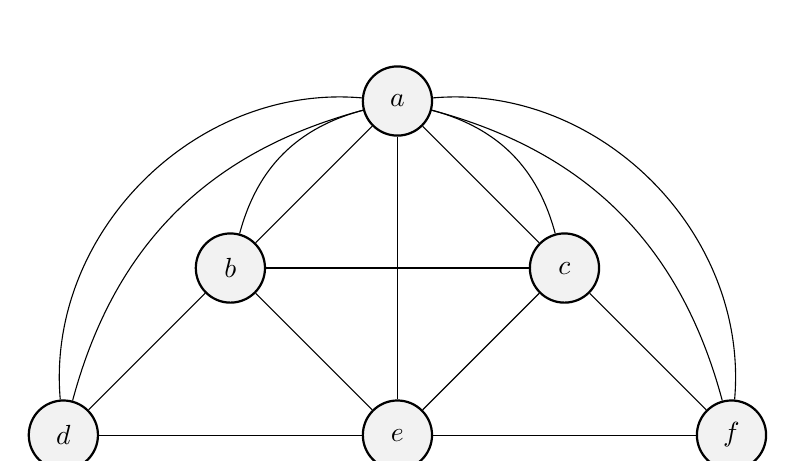
\begin{tikzpicture}
		\node[state] (1) {$a$};
		\node[state, below left of= 1] (2) {$b$};
		\node[state, below right of=1] (3) {$c$};
		\node[state, below left of=2] (4) {$d$};
		\node[state, below right of=2] (5) {$e$};
		\node[state, below right of=3] (6) {$f$};

		\draw 	(1) edge (2)
				(1) edge (3)
				(2) edge (3)
				(2) edge (4)
				(2) edge (5)
				(4) edge (5)
				(3) edge (5)
				(3) edge (6)
				(5) edge (6)
				(2) edge[bend left] (1)
				(3) edge[bend right] (1)
				(4) edge[bend left] (1)
				(4) edge[bend left=50] (1)
				(6) edge[bend right] (1)
				(6) edge[bend right=50] (1)
				(1) edge (5);
	\end{tikzpicture}
	\caption{Floor plan in graph form.}
	\label{floorplan}
\end{figure}

Also, apologies for the weird edge going from $e \rightarrow a$, I'm still trying to get used to tikz and I could not for the life of me figure out how to draw the edge around all the other nodes. If you have any tips, please let me know (it was a frustrating 1.5 hours of trying to get the edge to play nice before eventually giving up haha).

	
\end{document}